\section{Variantes}

\begin{frame}[fragile]{Solução linearítmica}

    \begin{itemize}
        \item A LIS pode ser encontrada por um algoritmo de programação dinâmica linearítmico

        \item Este algoritmo se baseia em um estado diferente do utilizado no algoritmo
            quadrático e em uma transição mais eficiente

        \item Seja $lis(k, i)$ o menor elemento que finaliza uma subsequência crescente de
            $\{ a_1, a_2, \ldots, a_i \}$ de tamanho $k$

        \item A segunda dimensão deste estado será implícita, sem necessidade de alocação de
            memória (caso contrário, a alocação da tabela de memória já tornaria este 
            algoritmo quadrático)

        \item Os casos bases acontecem com $i = 0$, isto é, antes de se considerar qualquer
            elemento da sequência

    \end{itemize}

\end{frame}

\begin{frame}[fragile]{Solução linearítmica}

    \begin{itemize}
        \item Para simplificar a implementação, pode-se fazer $lis(k, 0) = \infty$, para 
            todo $k\in [1, N]$ e $lis(0, 0) = 0$ (ou qualquer outro valor sentinela, desde
            que seja estritamente menor do que qualquer $a_i$)

        \item Para cada $i$, apenas um dos $lis(k, i)$ será atualizado

        \item Importante notar que os elementos da sequência $lis(1, i), lis(2, i), \ldots$
            estarão em ordem crescente

        \item Por meio de uma busca binária, deve-se identificar o primeiro índice $j$ tal que
            $lis(j, i - 1)$ seja estritamente maior do que $a_i$

        \item Daí, $lis(j, i) = a_i$

        \item O tamanho da lis será igual ao maior índice $j$ tal que $lis(j, N) < \infty$
    \end{itemize}

\end{frame}

\begin{frame}[fragile]{Visualização do algoritmo linearítmico para a LIS}

    \begin{figure}[h]
        \centering
        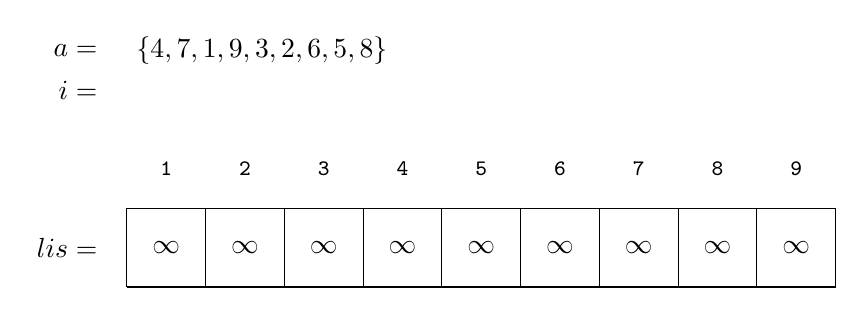
\begin{tikzpicture}

        \node[anchor=east] at (0.75, 4) { $a = $ };
        \node[anchor=west] at (1, 4) { $\{ 4, 7, 1, 9, 3, 2, 6, 5, 8 \}$ };
        \node[anchor=east] at (0.75, 3.5) { $i = $ };

        \node[anchor=east] at (0.75, 1.5) { $lis = $ };
        \draw (1, 1) grid (10, 2);

        \foreach \x in {1, ..., 9}
            \node at (\x + 0.5, 2.5) { \footnotesize \textbf{\texttt{\x}} };

        \node at (1.5, 1.5) { $\infty$ };
        \node at (2.5, 1.5) { $\infty$ };
        \node at (3.5, 1.5) { $\infty$ };
        \node at (4.5, 1.5) { $\infty$ };
        \node at (5.5, 1.5) { $\infty$ };
        \node at (6.5, 1.5) { $\infty$ };
        \node at (7.5, 1.5) { $\infty$ };
        \node at (8.5, 1.5) { $\infty$ };
        \node at (9.5, 1.5) { $\infty$ };
 
        \end{tikzpicture}
    \end{figure}

\end{frame}

\begin{frame}[fragile]{Visualização do algoritmo linearítmico para a LIS}

    \begin{figure}[h]
        \centering
        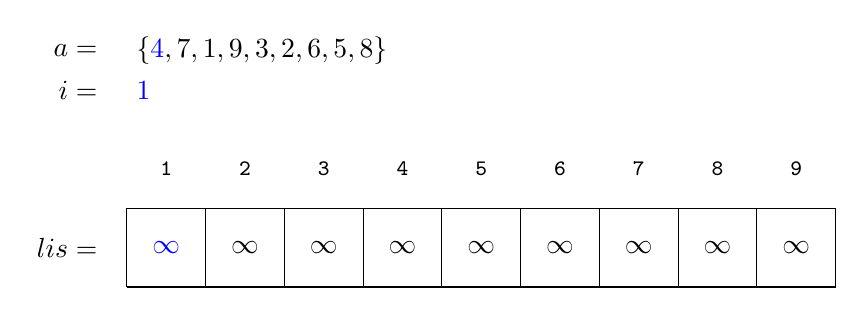
\begin{tikzpicture}

        \node[anchor=east] at (0.75, 4) { $a = $ };
        \node[anchor=west] at (1, 4) { $\{ \textcolor{blue}{4}, 7, 1, 9, 3, 2, 6, 5, 8 \}$ };
        \node[anchor=east] at (0.75, 3.5) { $i = $ };
        \node[anchor=west] at (1, 3.5) { $\textcolor{blue}{1}$ };

        \node[anchor=east] at (0.75, 1.5) { $lis = $ };
        \draw (1, 1) grid (10, 2);

        \foreach \x in {1, ..., 9}
            \node at (\x + 0.5, 2.5) { \footnotesize \textbf{\texttt{\x}} };

        \node at (1.5, 1.5) { \textcolor{blue}{$\infty$} };
        \node at (2.5, 1.5) { $\infty$ };
        \node at (3.5, 1.5) { $\infty$ };
        \node at (4.5, 1.5) { $\infty$ };
        \node at (5.5, 1.5) { $\infty$ };
        \node at (6.5, 1.5) { $\infty$ };
        \node at (7.5, 1.5) { $\infty$ };
        \node at (8.5, 1.5) { $\infty$ };
        \node at (9.5, 1.5) { $\infty$ };
 
        \end{tikzpicture}
    \end{figure}

\end{frame}

\begin{frame}[fragile]{Visualização do algoritmo linearítmico para a LIS}

    \begin{figure}[h]
        \centering
        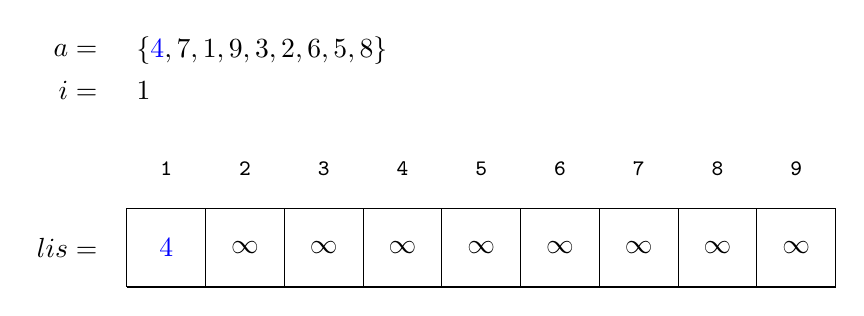
\begin{tikzpicture}

        \node[anchor=east] at (0.75, 4) { $a = $ };
        \node[anchor=west] at (1, 4) { $\{ \textcolor{blue}{4}, 7, 1, 9, 3, 2, 6, 5, 8 \}$ };
        \node[anchor=east] at (0.75, 3.5) { $i = $ };
        \node[anchor=west] at (1, 3.5) { $\textcolor{black}{1}$ };

        \node[anchor=east] at (0.75, 1.5) { $lis = $ };
        \draw (1, 1) grid (10, 2);

        \foreach \x in {1, ..., 9}
            \node at (\x + 0.5, 2.5) { \footnotesize \textbf{\texttt{\x}} };

        \node at (1.5, 1.5) { \textcolor{blue}{$4$} };
        \node at (2.5, 1.5) { $\infty$ };
        \node at (3.5, 1.5) { $\infty$ };
        \node at (4.5, 1.5) { $\infty$ };
        \node at (5.5, 1.5) { $\infty$ };
        \node at (6.5, 1.5) { $\infty$ };
        \node at (7.5, 1.5) { $\infty$ };
        \node at (8.5, 1.5) { $\infty$ };
        \node at (9.5, 1.5) { $\infty$ };
 
        \end{tikzpicture}
    \end{figure}

\end{frame}

\begin{frame}[fragile]{Visualização do algoritmo linearítmico para a LIS}

    \begin{figure}[h]
        \centering
        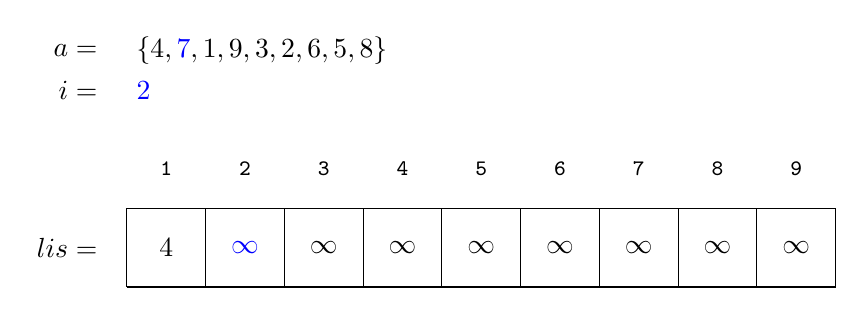
\begin{tikzpicture}

        \node[anchor=east] at (0.75, 4) { $a = $ };
        \node[anchor=west] at (1, 4) { $\{ \textcolor{black}{4}, \textcolor{blue}{7}, 1, 9, 3, 2, 6, 5, 8 \}$ };
        \node[anchor=east] at (0.75, 3.5) { $i = $ };
        \node[anchor=west] at (1, 3.5) { $\textcolor{blue}{2}$ };

        \node[anchor=east] at (0.75, 1.5) { $lis = $ };
        \draw (1, 1) grid (10, 2);

        \foreach \x in {1, ..., 9}
            \node at (\x + 0.5, 2.5) { \footnotesize \textbf{\texttt{\x}} };

        \node at (1.5, 1.5) { \textcolor{black}{$4$} };
        \node at (2.5, 1.5) { \textcolor{blue}{$\infty$} };
        \node at (3.5, 1.5) { $\infty$ };
        \node at (4.5, 1.5) { $\infty$ };
        \node at (5.5, 1.5) { $\infty$ };
        \node at (6.5, 1.5) { $\infty$ };
        \node at (7.5, 1.5) { $\infty$ };
        \node at (8.5, 1.5) { $\infty$ };
        \node at (9.5, 1.5) { $\infty$ };
 
        \end{tikzpicture}
    \end{figure}

\end{frame}

\begin{frame}[fragile]{Visualização do algoritmo linearítmico para a LIS}

    \begin{figure}[h]
        \centering
        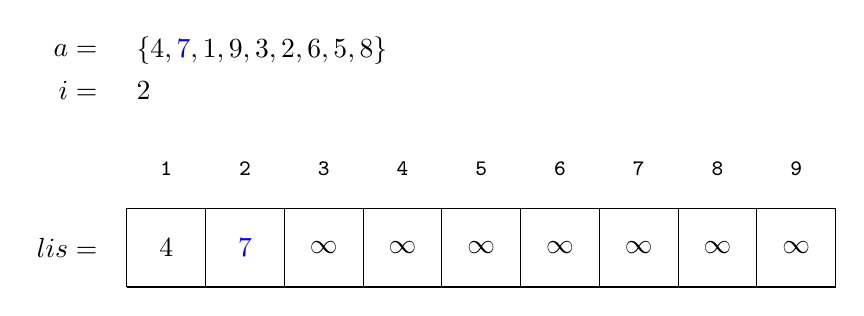
\begin{tikzpicture}

        \node[anchor=east] at (0.75, 4) { $a = $ };
        \node[anchor=west] at (1, 4) { $\{ \textcolor{black}{4}, \textcolor{blue}{7}, 1, 9, 3, 2, 6, 5, 8 \}$ };
        \node[anchor=east] at (0.75, 3.5) { $i = $ };
        \node[anchor=west] at (1, 3.5) { $\textcolor{black}{2}$ };

        \node[anchor=east] at (0.75, 1.5) { $lis = $ };
        \draw (1, 1) grid (10, 2);

        \foreach \x in {1, ..., 9}
            \node at (\x + 0.5, 2.5) { \footnotesize \textbf{\texttt{\x}} };

        \node at (1.5, 1.5) { \textcolor{black}{$4$} };
        \node at (2.5, 1.5) { \textcolor{blue}{$7$} };
        \node at (3.5, 1.5) { $\infty$ };
        \node at (4.5, 1.5) { $\infty$ };
        \node at (5.5, 1.5) { $\infty$ };
        \node at (6.5, 1.5) { $\infty$ };
        \node at (7.5, 1.5) { $\infty$ };
        \node at (8.5, 1.5) { $\infty$ };
        \node at (9.5, 1.5) { $\infty$ };
 
        \end{tikzpicture}
    \end{figure}

\end{frame}

\begin{frame}[fragile]{Visualização do algoritmo linearítmico para a LIS}

    \begin{figure}[h]
        \centering
        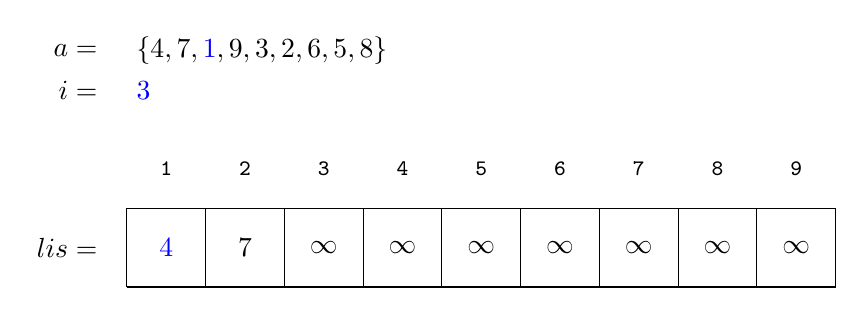
\begin{tikzpicture}

        \node[anchor=east] at (0.75, 4) { $a = $ };
        \node[anchor=west] at (1, 4) { $\{ \textcolor{black}{4}, \textcolor{black}{7}, \textcolor{blue}{1}, 9, 3, 2, 6, 5, 8 \}$ };
        \node[anchor=east] at (0.75, 3.5) { $i = $ };
        \node[anchor=west] at (1, 3.5) { $\textcolor{blue}{3}$ };

        \node[anchor=east] at (0.75, 1.5) { $lis = $ };
        \draw (1, 1) grid (10, 2);

        \foreach \x in {1, ..., 9}
            \node at (\x + 0.5, 2.5) { \footnotesize \textbf{\texttt{\x}} };

        \node at (1.5, 1.5) { \textcolor{blue}{$4$} };
        \node at (2.5, 1.5) { \textcolor{black}{$7$} };
        \node at (3.5, 1.5) { $\infty$ };
        \node at (4.5, 1.5) { $\infty$ };
        \node at (5.5, 1.5) { $\infty$ };
        \node at (6.5, 1.5) { $\infty$ };
        \node at (7.5, 1.5) { $\infty$ };
        \node at (8.5, 1.5) { $\infty$ };
        \node at (9.5, 1.5) { $\infty$ };
 
        \end{tikzpicture}
    \end{figure}

\end{frame}

\begin{frame}[fragile]{Visualização do algoritmo linearítmico para a LIS}

    \begin{figure}[h]
        \centering
        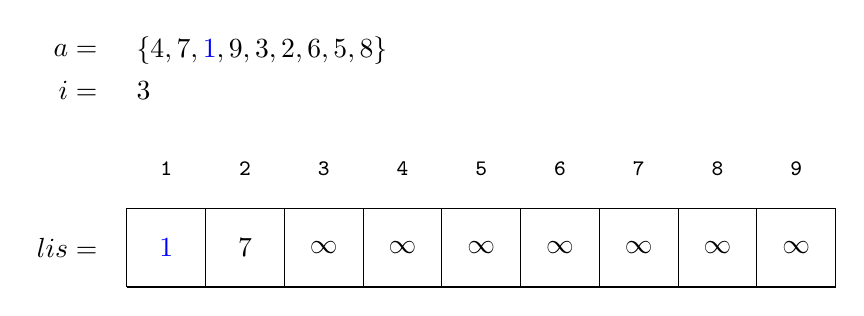
\begin{tikzpicture}

        \node[anchor=east] at (0.75, 4) { $a = $ };
        \node[anchor=west] at (1, 4) { $\{ \textcolor{black}{4}, \textcolor{black}{7}, \textcolor{blue}{1}, 9, 3, 2, 6, 5, 8 \}$ };
        \node[anchor=east] at (0.75, 3.5) { $i = $ };
        \node[anchor=west] at (1, 3.5) { $\textcolor{black}{3}$ };

        \node[anchor=east] at (0.75, 1.5) { $lis = $ };
        \draw (1, 1) grid (10, 2);

        \foreach \x in {1, ..., 9}
            \node at (\x + 0.5, 2.5) { \footnotesize \textbf{\texttt{\x}} };

        \node at (1.5, 1.5) { \textcolor{blue}{$1$} };
        \node at (2.5, 1.5) { \textcolor{black}{$7$} };
        \node at (3.5, 1.5) { $\infty$ };
        \node at (4.5, 1.5) { $\infty$ };
        \node at (5.5, 1.5) { $\infty$ };
        \node at (6.5, 1.5) { $\infty$ };
        \node at (7.5, 1.5) { $\infty$ };
        \node at (8.5, 1.5) { $\infty$ };
        \node at (9.5, 1.5) { $\infty$ };
 
        \end{tikzpicture}
    \end{figure}

\end{frame}

\begin{frame}[fragile]{Visualização do algoritmo linearítmico para a LIS}

    \begin{figure}[h]
        \centering
        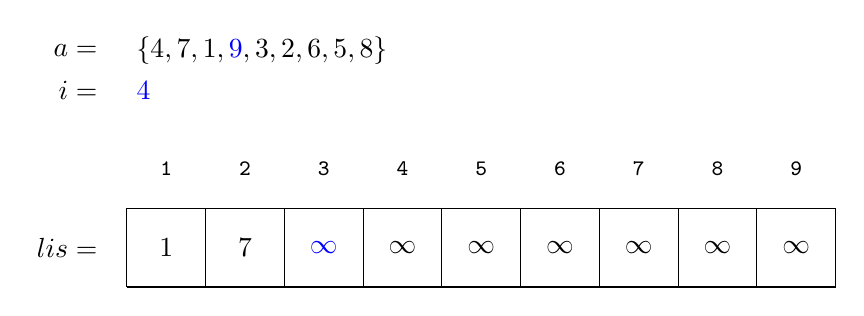
\begin{tikzpicture}

        \node[anchor=east] at (0.75, 4) { $a = $ };
        \node[anchor=west] at (1, 4) { $\{ \textcolor{black}{4}, \textcolor{black}{7}, \textcolor{black}{1}, \textcolor{blue}{9}, 3, 2, 6, 5, 8 \}$ };
        \node[anchor=east] at (0.75, 3.5) { $i = $ };
        \node[anchor=west] at (1, 3.5) { $\textcolor{blue}{4}$ };

        \node[anchor=east] at (0.75, 1.5) { $lis = $ };
        \draw (1, 1) grid (10, 2);

        \foreach \x in {1, ..., 9}
            \node at (\x + 0.5, 2.5) { \footnotesize \textbf{\texttt{\x}} };

        \node at (1.5, 1.5) { \textcolor{black}{$1$} };
        \node at (2.5, 1.5) { \textcolor{black}{$7$} };
        \node at (3.5, 1.5) { \textcolor{blue}{$\infty$} };
        \node at (4.5, 1.5) { $\infty$ };
        \node at (5.5, 1.5) { $\infty$ };
        \node at (6.5, 1.5) { $\infty$ };
        \node at (7.5, 1.5) { $\infty$ };
        \node at (8.5, 1.5) { $\infty$ };
        \node at (9.5, 1.5) { $\infty$ };
 
        \end{tikzpicture}
    \end{figure}

\end{frame}

\begin{frame}[fragile]{Visualização do algoritmo linearítmico para a LIS}

    \begin{figure}[h]
        \centering
        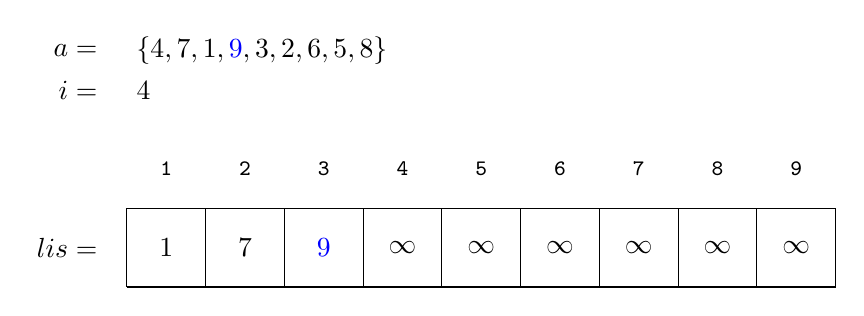
\begin{tikzpicture}

        \node[anchor=east] at (0.75, 4) { $a = $ };
        \node[anchor=west] at (1, 4) { $\{ \textcolor{black}{4}, \textcolor{black}{7}, \textcolor{black}{1}, \textcolor{blue}{9}, 3, 2, 6, 5, 8 \}$ };
        \node[anchor=east] at (0.75, 3.5) { $i = $ };
        \node[anchor=west] at (1, 3.5) { $\textcolor{black}{4}$ };

        \node[anchor=east] at (0.75, 1.5) { $lis = $ };
        \draw (1, 1) grid (10, 2);

        \foreach \x in {1, ..., 9}
            \node at (\x + 0.5, 2.5) { \footnotesize \textbf{\texttt{\x}} };

        \node at (1.5, 1.5) { \textcolor{black}{$1$} };
        \node at (2.5, 1.5) { \textcolor{black}{$7$} };
        \node at (3.5, 1.5) { \textcolor{blue}{$9$} };
        \node at (4.5, 1.5) { $\infty$ };
        \node at (5.5, 1.5) { $\infty$ };
        \node at (6.5, 1.5) { $\infty$ };
        \node at (7.5, 1.5) { $\infty$ };
        \node at (8.5, 1.5) { $\infty$ };
        \node at (9.5, 1.5) { $\infty$ };
 
        \end{tikzpicture}
    \end{figure}

\end{frame}

\begin{frame}[fragile]{Visualização do algoritmo linearítmico para a LIS}

    \begin{figure}[h]
        \centering
        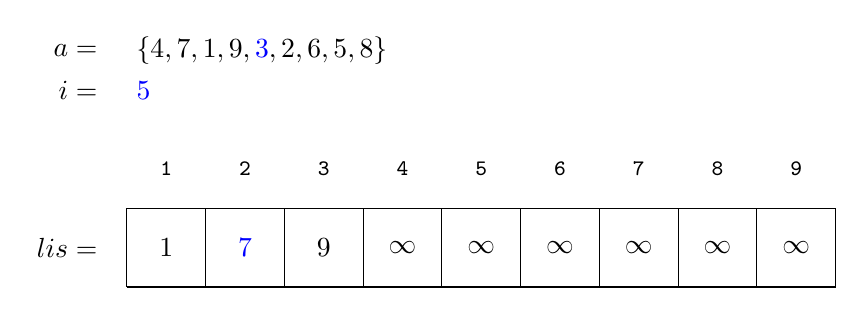
\begin{tikzpicture}

        \node[anchor=east] at (0.75, 4) { $a = $ };
        \node[anchor=west] at (1, 4) { $\{ \textcolor{black}{4}, \textcolor{black}{7}, \textcolor{black}{1}, \textcolor{black}{9}, \textcolor{blue}{3}, 2, 6, 5, 8 \}$ };
        \node[anchor=east] at (0.75, 3.5) { $i = $ };
        \node[anchor=west] at (1, 3.5) { $\textcolor{blue}{5}$ };

        \node[anchor=east] at (0.75, 1.5) { $lis = $ };
        \draw (1, 1) grid (10, 2);

        \foreach \x in {1, ..., 9}
            \node at (\x + 0.5, 2.5) { \footnotesize \textbf{\texttt{\x}} };

        \node at (1.5, 1.5) { \textcolor{black}{$1$} };
        \node at (2.5, 1.5) { \textcolor{blue}{$7$} };
        \node at (3.5, 1.5) { \textcolor{black}{$9$} };
        \node at (4.5, 1.5) { $\infty$ };
        \node at (5.5, 1.5) { $\infty$ };
        \node at (6.5, 1.5) { $\infty$ };
        \node at (7.5, 1.5) { $\infty$ };
        \node at (8.5, 1.5) { $\infty$ };
        \node at (9.5, 1.5) { $\infty$ };
 
        \end{tikzpicture}
    \end{figure}

\end{frame}

\begin{frame}[fragile]{Visualização do algoritmo linearítmico para a LIS}

    \begin{figure}[h]
        \centering
        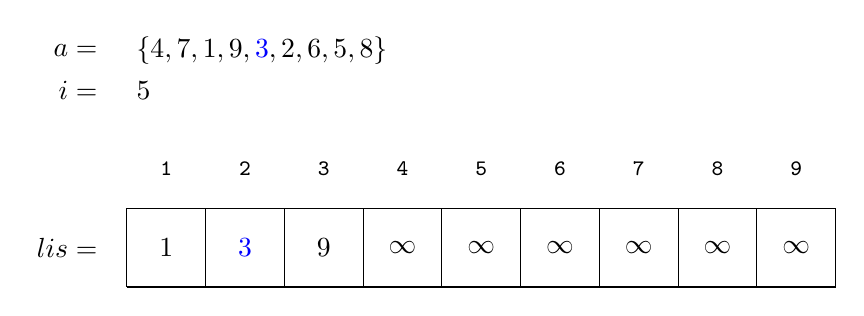
\begin{tikzpicture}

        \node[anchor=east] at (0.75, 4) { $a = $ };
        \node[anchor=west] at (1, 4) { $\{ \textcolor{black}{4}, \textcolor{black}{7}, \textcolor{black}{1}, \textcolor{black}{9}, \textcolor{blue}{3}, 2, 6, 5, 8 \}$ };
        \node[anchor=east] at (0.75, 3.5) { $i = $ };
        \node[anchor=west] at (1, 3.5) { $\textcolor{black}{5}$ };

        \node[anchor=east] at (0.75, 1.5) { $lis = $ };
        \draw (1, 1) grid (10, 2);

        \foreach \x in {1, ..., 9}
            \node at (\x + 0.5, 2.5) { \footnotesize \textbf{\texttt{\x}} };

        \node at (1.5, 1.5) { \textcolor{black}{$1$} };
        \node at (2.5, 1.5) { \textcolor{blue}{$3$} };
        \node at (3.5, 1.5) { \textcolor{black}{$9$} };
        \node at (4.5, 1.5) { $\infty$ };
        \node at (5.5, 1.5) { $\infty$ };
        \node at (6.5, 1.5) { $\infty$ };
        \node at (7.5, 1.5) { $\infty$ };
        \node at (8.5, 1.5) { $\infty$ };
        \node at (9.5, 1.5) { $\infty$ };
 
        \end{tikzpicture}
    \end{figure}

\end{frame}

\begin{frame}[fragile]{Visualização do algoritmo linearítmico para a LIS}

    \begin{figure}[h]
        \centering
        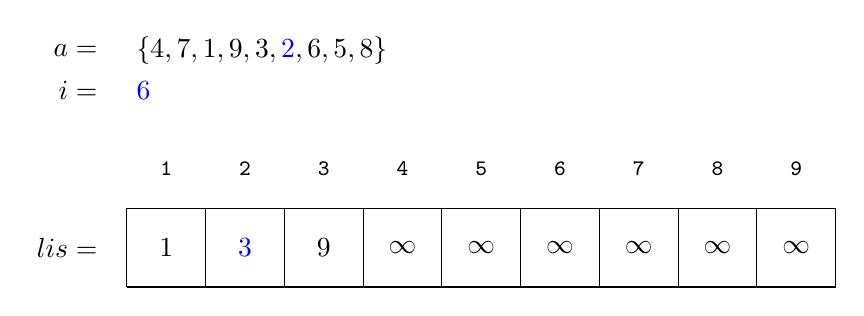
\begin{tikzpicture}

        \node[anchor=east] at (0.75, 4) { $a = $ };
        \node[anchor=west] at (1, 4) { $\{ \textcolor{black}{4}, \textcolor{black}{7}, \textcolor{black}{1}, \textcolor{black}{9}, \textcolor{black}{3}, \textcolor{blue}{2}, 6, 5, 8 \}$ };
        \node[anchor=east] at (0.75, 3.5) { $i = $ };
        \node[anchor=west] at (1, 3.5) { $\textcolor{blue}{6}$ };

        \node[anchor=east] at (0.75, 1.5) { $lis = $ };
        \draw (1, 1) grid (10, 2);

        \foreach \x in {1, ..., 9}
            \node at (\x + 0.5, 2.5) { \footnotesize \textbf{\texttt{\x}} };

        \node at (1.5, 1.5) { \textcolor{black}{$1$} };
        \node at (2.5, 1.5) { \textcolor{blue}{$3$} };
        \node at (3.5, 1.5) { \textcolor{black}{$9$} };
        \node at (4.5, 1.5) { $\infty$ };
        \node at (5.5, 1.5) { $\infty$ };
        \node at (6.5, 1.5) { $\infty$ };
        \node at (7.5, 1.5) { $\infty$ };
        \node at (8.5, 1.5) { $\infty$ };
        \node at (9.5, 1.5) { $\infty$ };
 
        \end{tikzpicture}
    \end{figure}

\end{frame}

\begin{frame}[fragile]{Visualização do algoritmo linearítmico para a LIS}

    \begin{figure}[h]
        \centering
        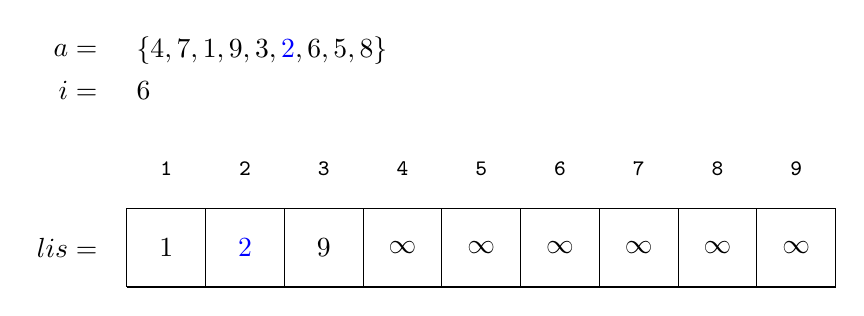
\begin{tikzpicture}

        \node[anchor=east] at (0.75, 4) { $a = $ };
        \node[anchor=west] at (1, 4) { $\{ \textcolor{black}{4}, \textcolor{black}{7}, \textcolor{black}{1}, \textcolor{black}{9}, \textcolor{black}{3}, \textcolor{blue}{2}, 6, 5, 8 \}$ };
        \node[anchor=east] at (0.75, 3.5) { $i = $ };
        \node[anchor=west] at (1, 3.5) { $\textcolor{black}{6}$ };

        \node[anchor=east] at (0.75, 1.5) { $lis = $ };
        \draw (1, 1) grid (10, 2);

        \foreach \x in {1, ..., 9}
            \node at (\x + 0.5, 2.5) { \footnotesize \textbf{\texttt{\x}} };

        \node at (1.5, 1.5) { \textcolor{black}{$1$} };
        \node at (2.5, 1.5) { \textcolor{blue}{$2$} };
        \node at (3.5, 1.5) { \textcolor{black}{$9$} };
        \node at (4.5, 1.5) { $\infty$ };
        \node at (5.5, 1.5) { $\infty$ };
        \node at (6.5, 1.5) { $\infty$ };
        \node at (7.5, 1.5) { $\infty$ };
        \node at (8.5, 1.5) { $\infty$ };
        \node at (9.5, 1.5) { $\infty$ };
 
        \end{tikzpicture}
    \end{figure}

\end{frame}

\begin{frame}[fragile]{Visualização do algoritmo linearítmico para a LIS}

    \begin{figure}[h]
        \centering
        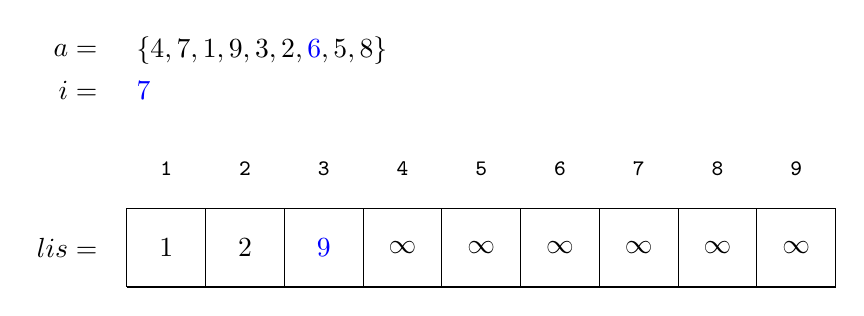
\begin{tikzpicture}

        \node[anchor=east] at (0.75, 4) { $a = $ };
        \node[anchor=west] at (1, 4) { $\{ \textcolor{black}{4}, \textcolor{black}{7}, \textcolor{black}{1}, \textcolor{black}{9}, \textcolor{black}{3}, \textcolor{black}{2}, \textcolor{blue}{6}, 5, 8 \}$ };
        \node[anchor=east] at (0.75, 3.5) { $i = $ };
        \node[anchor=west] at (1, 3.5) { $\textcolor{blue}{7}$ };

        \node[anchor=east] at (0.75, 1.5) { $lis = $ };
        \draw (1, 1) grid (10, 2);

        \foreach \x in {1, ..., 9}
            \node at (\x + 0.5, 2.5) { \footnotesize \textbf{\texttt{\x}} };

        \node at (1.5, 1.5) { \textcolor{black}{$1$} };
        \node at (2.5, 1.5) { \textcolor{black}{$2$} };
        \node at (3.5, 1.5) { \textcolor{blue}{$9$} };
        \node at (4.5, 1.5) { $\infty$ };
        \node at (5.5, 1.5) { $\infty$ };
        \node at (6.5, 1.5) { $\infty$ };
        \node at (7.5, 1.5) { $\infty$ };
        \node at (8.5, 1.5) { $\infty$ };
        \node at (9.5, 1.5) { $\infty$ };
 
        \end{tikzpicture}
    \end{figure}

\end{frame}

\begin{frame}[fragile]{Visualização do algoritmo linearítmico para a LIS}

    \begin{figure}[h]
        \centering
        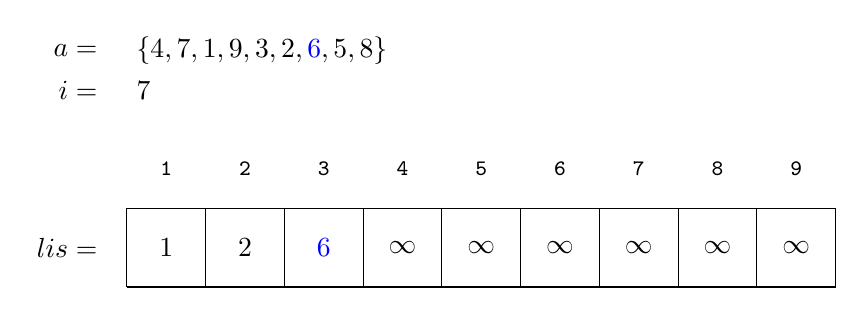
\begin{tikzpicture}

        \node[anchor=east] at (0.75, 4) { $a = $ };
        \node[anchor=west] at (1, 4) { $\{ \textcolor{black}{4}, \textcolor{black}{7}, \textcolor{black}{1}, \textcolor{black}{9}, \textcolor{black}{3}, \textcolor{black}{2}, \textcolor{blue}{6}, 5, 8 \}$ };
        \node[anchor=east] at (0.75, 3.5) { $i = $ };
        \node[anchor=west] at (1, 3.5) { $\textcolor{black}{7}$ };

        \node[anchor=east] at (0.75, 1.5) { $lis = $ };
        \draw (1, 1) grid (10, 2);

        \foreach \x in {1, ..., 9}
            \node at (\x + 0.5, 2.5) { \footnotesize \textbf{\texttt{\x}} };

        \node at (1.5, 1.5) { \textcolor{black}{$1$} };
        \node at (2.5, 1.5) { \textcolor{black}{$2$} };
        \node at (3.5, 1.5) { \textcolor{blue}{$6$} };
        \node at (4.5, 1.5) { $\infty$ };
        \node at (5.5, 1.5) { $\infty$ };
        \node at (6.5, 1.5) { $\infty$ };
        \node at (7.5, 1.5) { $\infty$ };
        \node at (8.5, 1.5) { $\infty$ };
        \node at (9.5, 1.5) { $\infty$ };
 
        \end{tikzpicture}
    \end{figure}

\end{frame}

\begin{frame}[fragile]{Visualização do algoritmo linearítmico para a LIS}

    \begin{figure}[h]
        \centering
        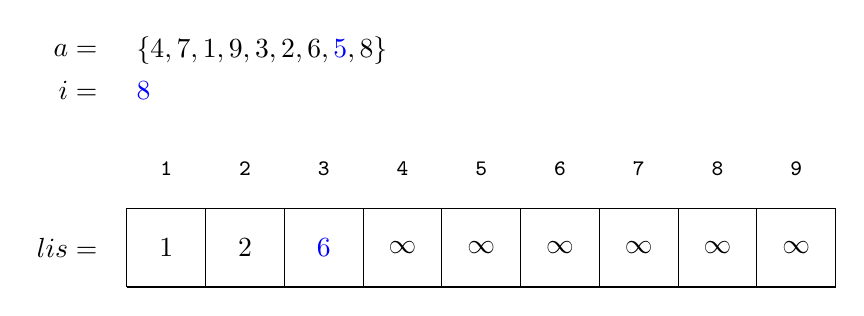
\begin{tikzpicture}

        \node[anchor=east] at (0.75, 4) { $a = $ };
        \node[anchor=west] at (1, 4) { $\{ \textcolor{black}{4}, \textcolor{black}{7}, \textcolor{black}{1}, \textcolor{black}{9}, \textcolor{black}{3}, \textcolor{black}{2}, \textcolor{black}{6}, \textcolor{blue}{5}, 8 \}$ };
        \node[anchor=east] at (0.75, 3.5) { $i = $ };
        \node[anchor=west] at (1, 3.5) { $\textcolor{blue}{8}$ };

        \node[anchor=east] at (0.75, 1.5) { $lis = $ };
        \draw (1, 1) grid (10, 2);

        \foreach \x in {1, ..., 9}
            \node at (\x + 0.5, 2.5) { \footnotesize \textbf{\texttt{\x}} };

        \node at (1.5, 1.5) { \textcolor{black}{$1$} };
        \node at (2.5, 1.5) { \textcolor{black}{$2$} };
        \node at (3.5, 1.5) { \textcolor{blue}{$6$} };
        \node at (4.5, 1.5) { $\infty$ };
        \node at (5.5, 1.5) { $\infty$ };
        \node at (6.5, 1.5) { $\infty$ };
        \node at (7.5, 1.5) { $\infty$ };
        \node at (8.5, 1.5) { $\infty$ };
        \node at (9.5, 1.5) { $\infty$ };
 
        \end{tikzpicture}
    \end{figure}

\end{frame}

\begin{frame}[fragile]{Visualização do algoritmo linearítmico para a LIS}

    \begin{figure}[h]
        \centering
        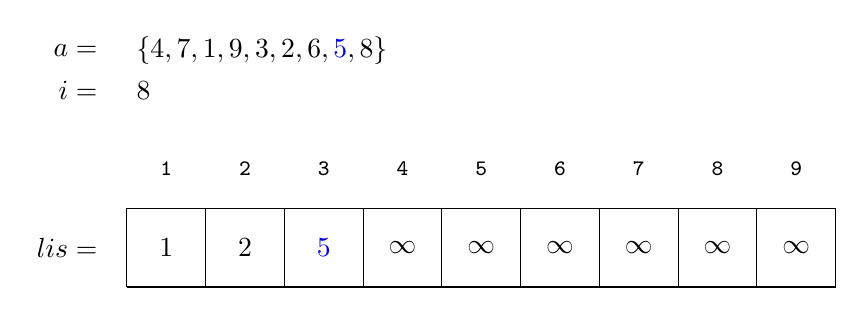
\begin{tikzpicture}

        \node[anchor=east] at (0.75, 4) { $a = $ };
        \node[anchor=west] at (1, 4) { $\{ \textcolor{black}{4}, \textcolor{black}{7}, \textcolor{black}{1}, \textcolor{black}{9}, \textcolor{black}{3}, \textcolor{black}{2}, \textcolor{black}{6}, \textcolor{blue}{5}, 8 \}$ };
        \node[anchor=east] at (0.75, 3.5) { $i = $ };
        \node[anchor=west] at (1, 3.5) { $\textcolor{black}{8}$ };

        \node[anchor=east] at (0.75, 1.5) { $lis = $ };
        \draw (1, 1) grid (10, 2);

        \foreach \x in {1, ..., 9}
            \node at (\x + 0.5, 2.5) { \footnotesize \textbf{\texttt{\x}} };

        \node at (1.5, 1.5) { \textcolor{black}{$1$} };
        \node at (2.5, 1.5) { \textcolor{black}{$2$} };
        \node at (3.5, 1.5) { \textcolor{blue}{$5$} };
        \node at (4.5, 1.5) { $\infty$ };
        \node at (5.5, 1.5) { $\infty$ };
        \node at (6.5, 1.5) { $\infty$ };
        \node at (7.5, 1.5) { $\infty$ };
        \node at (8.5, 1.5) { $\infty$ };
        \node at (9.5, 1.5) { $\infty$ };
 
        \end{tikzpicture}
    \end{figure}

\end{frame}

\begin{frame}[fragile]{Visualização do algoritmo linearítmico para a LIS}

    \begin{figure}[h]
        \centering
        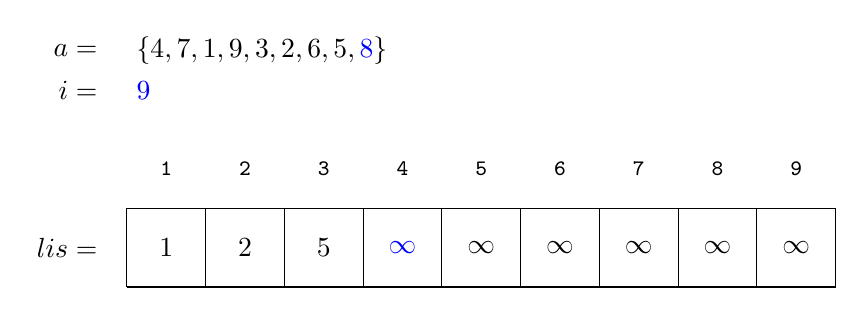
\begin{tikzpicture}

        \node[anchor=east] at (0.75, 4) { $a = $ };
        \node[anchor=west] at (1, 4) { $\{ \textcolor{black}{4}, \textcolor{black}{7}, \textcolor{black}{1}, \textcolor{black}{9}, \textcolor{black}{3}, \textcolor{black}{2}, \textcolor{black}{6}, \textcolor{black}{5}, \textcolor{blue}{8} \}$ };
        \node[anchor=east] at (0.75, 3.5) { $i = $ };
        \node[anchor=west] at (1, 3.5) { $\textcolor{blue}{9}$ };

        \node[anchor=east] at (0.75, 1.5) { $lis = $ };
        \draw (1, 1) grid (10, 2);

        \foreach \x in {1, ..., 9}
            \node at (\x + 0.5, 2.5) { \footnotesize \textbf{\texttt{\x}} };

        \node at (1.5, 1.5) { \textcolor{black}{$1$} };
        \node at (2.5, 1.5) { \textcolor{black}{$2$} };
        \node at (3.5, 1.5) { \textcolor{black}{$5$} };
        \node at (4.5, 1.5) { \textcolor{blue}{$\infty$} };
        \node at (5.5, 1.5) { $\infty$ };
        \node at (6.5, 1.5) { $\infty$ };
        \node at (7.5, 1.5) { $\infty$ };
        \node at (8.5, 1.5) { $\infty$ };
        \node at (9.5, 1.5) { $\infty$ };
 
        \end{tikzpicture}
    \end{figure}

\end{frame}

\begin{frame}[fragile]{Visualização do algoritmo linearítmico para a LIS}

    \begin{figure}[h]
        \centering
        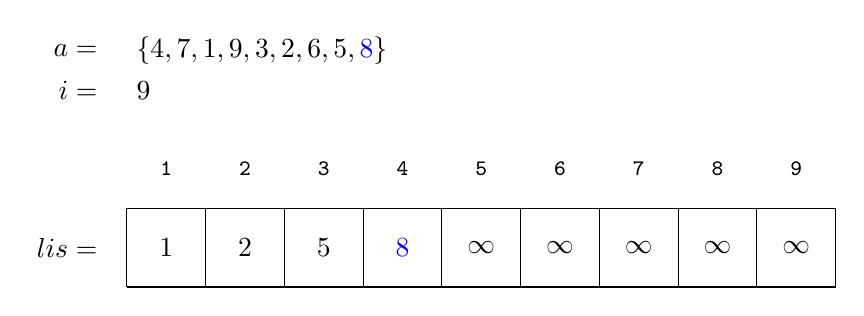
\begin{tikzpicture}

        \node[anchor=east] at (0.75, 4) { $a = $ };
        \node[anchor=west] at (1, 4) { $\{ \textcolor{black}{4}, \textcolor{black}{7}, \textcolor{black}{1}, \textcolor{black}{9}, \textcolor{black}{3}, \textcolor{black}{2}, \textcolor{black}{6}, \textcolor{black}{5}, \textcolor{blue}{8} \}$ };
        \node[anchor=east] at (0.75, 3.5) { $i = $ };
        \node[anchor=west] at (1, 3.5) { $\textcolor{black}{9}$ };

        \node[anchor=east] at (0.75, 1.5) { $lis = $ };
        \draw (1, 1) grid (10, 2);

        \foreach \x in {1, ..., 9}
            \node at (\x + 0.5, 2.5) { \footnotesize \textbf{\texttt{\x}} };

        \node at (1.5, 1.5) { \textcolor{black}{$1$} };
        \node at (2.5, 1.5) { \textcolor{black}{$2$} };
        \node at (3.5, 1.5) { \textcolor{black}{$5$} };
        \node at (4.5, 1.5) { \textcolor{blue}{$8$} };
        \node at (5.5, 1.5) { $\infty$ };
        \node at (6.5, 1.5) { $\infty$ };
        \node at (7.5, 1.5) { $\infty$ };
        \node at (8.5, 1.5) { $\infty$ };
        \node at (9.5, 1.5) { $\infty$ };
 
        \end{tikzpicture}
    \end{figure}

\end{frame}


\begin{frame}[fragile]{Implementação linearítmica da LIS}
    \inputsnippet{cpp}{5}{24}{codes/lis_linearitmico.cpp}
\end{frame}
